\documentclass[11pt,a4paper]{article}

\usepackage[utf8]{inputenc}
\usepackage[T1]{fontenc}
\usepackage[margin=1in]{geometry}
\usepackage{amsmath,amssymb}
\usepackage{booktabs}
\usepackage{graphicx}
\usepackage{xcolor}
\definecolor{firstbest}{rgb}{0.8, 0.0, 0.0}
\definecolor{secondbest}{rgb}{0.0, 0.0, 0.8}
\newcommand{\first}[1]{\textcolor{firstbest}{\textbf{#1}}}
\newcommand{\second}[1]{\textcolor{secondbest}{\textbf{#1}}}
\usepackage{enumitem}
\usepackage{tikz}
\usetikzlibrary{arrows.meta,positioning,fit,calc,shapes.geometric,backgrounds}
\usepackage[hidelinks]{hyperref}

\newcommand{\Binf}{B_\infty}
\newcommand{\J}{J}
\newcommand{\I}{I}
\newcommand{\sg}{\operatorname{sg}}
\newcommand{\Lcal}{\mathcal{L}}

\title{\textbf{PhysDecouple-4DGS: Direct Underwater Rendering with Physics-Decoupled 4D Gaussian Splatting for Dynamic Scene Restoration and Transient Distractor Removal}}
\author{ME21B171}
\date{June 2026}

\begin{document}

\maketitle

\begin{abstract}
Monocular underwater video entangles three phenomena that existing novel-view synthesis methods treat in isolation: a \emph{dynamic} scene, a range-dependent \emph{scattering medium}, and \emph{transient distractors} that occlude the scene of interest. We introduce PhysDecouple-4DGS, a direct underwater rendering framework that factorizes all three from a single video. A deformable Gaussian scene representation renders the latent water-free radiance $\J$ together with per-pixel range; a compact, physically constrained medium model (19 scalar parameters) composites the underwater observation $\I$ through the revised image formation model, and supervision is applied exclusively to $\I$. Restoration is thus obtained by \emph{reading out} $\J$ rather than by inverting the formation equation, which is ill-conditioned at low transmission. The central challenge is identifiability: the data admit a continuum of scene--medium explanations. We resolve it with three mechanisms. First, the veiling light $\Binf$ is \emph{measured} from open-water rays --- rays that the reconstruction marks as hitting no geometry observe the water column, whose radiance converges to $\Binf$ --- which bounds backscatter compensation by the true veil. Second, the spectral structure of attenuation and backscatter is enforced \emph{by construction} through ordered, bounded reparameterizations rather than penalties. Third, we introduce a \emph{depth--chromaticity decorrelation} objective derived from a necessary condition on any correct restoration: since the medium is the only range-dependent term in the formation model, restored chromaticity must be statistically independent of range. This criterion is hue-agnostic and water-type-agnostic, and subsumes the color-cast failure modes (blue, green, yellow, red) reported across prior underwater restoration work. Transients are modeled by a per-Gaussian transient probability trained from rendering residuals; it gates the photometric loss so distractors are never absorbed into the representation, and supports test-time suppression. One trained model renders reconstruction and restoration, each with and without transients, and additionally supports static-scene extraction by suppressing the learned dynamics.
\end{abstract}

\section{Introduction}

Restoring underwater imagery requires inverting a range-dependent physical degradation; reconstructing a dynamic scene requires attributing image motion to scene deformation; and removing distractors requires deciding which observations belong to the scene at all. In monocular underwater video these problems are coupled through every pixel: a fish, the veil of water behind it, and the swaying vegetation it occludes all contribute to the same observation. Methods that address only one factor implicitly push the remaining factors into whichever representation is most flexible --- typically the scene model \cite{mildenhall2020nerf,kerbl20233d} --- where they reappear as color casts, fog-like geometry, or view-inconsistent artifacts.

Our guiding principle is \emph{decoupling by construction}: each physical factor is represented by a module whose capacity and parameterization restrict it to that factor, and every quantity that is observable from the data is estimated by measurement rather than left to gradient descent. The scene is a deformable Gaussian representation that can only express geometry, appearance, and temporally coherent motion; the medium is a 19-parameter optical model that can only express range-dependent attenuation and backscatter consistent with oceanographic constraints; transients are carried by a dedicated per-Gaussian channel trained from the model's own rendering residuals.

\paragraph{Contributions.}
\begin{enumerate}[leftmargin=1.2cm,itemsep=2pt]
    \item \textbf{Direct underwater rendering for dynamic scenes.} In the spirit of Gaussian-Splashing-style direct rendering \cite{mualem2024gaussiansplashing}, the latent clean radiance $\J$ and range $\bar d$ are rasterized from a deformable Gaussian representation \cite{wu20244d}, and a differentiable forward medium composites the underwater prediction $\I$ for supervision (Sec.~\ref{sec:dur}). The restoration is the latent image itself; no per-frame inversion is ever performed.
    \item \textbf{A compact, physically constrained medium.} We replace spatio-temporal coefficient grids with a 19-parameter model --- a two-term exponential range profile per channel for direct attenuation ($3{\times}4$), scene-constant backscatter and veiling-light chromaticities ($3{+}3$), and one bounded optical-path scale --- whose Jerlov spectral orderings \cite{jerlov1976marine} hold by construction at every range (Sec.~\ref{sec:medium-param}).
    \item \textbf{Measurement-first estimation of the medium.} The veiling light is measured from open-water rays; the remaining medium parameters are pre-calibrated against the data before joint optimization begins. Both steps follow directly from the formation model and remove the dominant ambiguity of the scene--medium decomposition (Sec.~\ref{sec:measurement}).
    \item \textbf{Depth--chromaticity decorrelation.} A necessary condition on correct restoration --- restored chromaticity is independent of range --- expressed as a training objective. The criterion involves no reference colors, no water-type assumptions, and no per-scene constants, and addresses the full family of depth-graded color casts \cite{akkaynak2019sea,levy2023seathru} with a single term (Sec.~\ref{sec:losses}).
    \item \textbf{A three-way motion taxonomy with residual-driven transient modeling.} The framework distinguishes persistent static structure, persistent dynamics (modeled by the deformation field \cite{pumarola2021d,wu20244d}), and transients (carried by a per-Gaussian probability $\sigma$ trained via residual-guided spatial assignment). $\sigma$ gates the photometric loss during training, so distractors never enter the scene representation, and gates opacity at test time for suppression; a complementary motion gate extracts the static scene (Sec.~\ref{sec:transients}).
    \item \textbf{An identifiability-aware optimization schedule}, including a stop-gradient between rendered range and the medium exponentials, medium-first adaptation, and a separation of auxiliary objectives into ungated \emph{anchors} and quality-gated \emph{refinements}, each justified by an explicit failure mode of the naive joint problem (Secs.~\ref{sec:opt},~\ref{sec:analysis}).
\end{enumerate}

\section{Direct Underwater Rendering}
\label{sec:dur}

\subsection{Image formation}

For color channel $c \in \{R,G,B\}$ and camera--object range $d$, the revised underwater image formation model \cite{akkaynak2018revised} expresses the observation as the sum of an attenuated signal and accumulated backscatter:
\begin{equation}
    \I^c(\mathbf{x})
    =
    \J^c(\mathbf{x})\; e^{-\beta_D^c(z)\, d(\mathbf{x})}
    \;+\;
    \Binf^c \left(1-e^{-\beta_B^c\, d(\mathbf{x})}\right),
    \label{eq:forward}
\end{equation}
with clean radiance $\J$, direct attenuation coefficients $\beta_D^c(z)$ (range-dependent), backscatter coefficients $\beta_B^c$, and veiling light $\Binf^c$. The classical restoration route inverts Eq.~\eqref{eq:forward} per image; because the inverse multiplies by $e^{+\beta_D d}$, estimation error in range or coefficients is amplified exponentially exactly where the water is thickest. Direct underwater rendering avoids the inverse entirely: the scene representation renders $\J$, Eq.~\eqref{eq:forward} is evaluated \emph{forward} inside the differentiable rasterization pipeline, and the photometric loss compares $\I$ with the observation $\I^\star$. Under this composition the medium parameters are the only mechanism by which water can affect the prediction, so the optimum places the water in the medium and the scene in $\J$.

\subsection{Scene representation}

The scene is a set of anisotropic 3D Gaussians $\{\boldsymbol{\mu}_i, \boldsymbol{\Sigma}_i, \alpha_i, \mathbf{c}_i, s_i\}$ with spherical-harmonics appearance $\mathbf{c}_i$ \cite{kerbl20233d} and a transient logit $s_i$, deformed in time by a HexPlane field $\mathcal{D}_\theta$ \cite{cao2023hexplane,wu20244d}:
\begin{equation}
    (\boldsymbol{\mu}_i^t, \mathbf{s}_i^t, \mathbf{R}_i^t) = \mathcal{D}_\theta(\boldsymbol{\mu}_i, \mathbf{s}_i, \mathbf{R}_i, t).
\end{equation}
A single rasterization pass produces three aligned maps: the clean render $\J$ (straight-through clamped to valid radiance), the expected range $\bar d \in [0,1]$ (alpha-normalized, converted from $z$-depth to optical path length, normalized by a robust scene maximum), and the transient map $\sigma(\mathbf{x})$ obtained by rasterizing $\sigma_i = \mathrm{sigmoid}(s_i)$ as the splatted quantity.

\paragraph{Range as data: stop-gradient into the medium.}
The composition consumes $\sg[\bar d\,]$ --- range with the gradient detached. Allowing $\partial \I / \partial \bar d$ to reach the geometry turns per-pixel range into an unconstrained color control: the optimizer lowers photometric error by fragmenting geometry into micro-floaters whose depths modulate the exponentials (``depth painting''), and gradient-magnitude-driven densification multiplies them. With the stop-gradient, geometry is shaped only by the radiance pathway and by explicit range supervision: a scale/shift-invariant correlation loss against monocular depth and an edge-aware smoothness term (Sec.~\ref{sec:losses}).

\section{A Compact Physically Constrained Medium}
\label{sec:medium-param}

Earlier iterations of this work parameterized the medium as depth--time coefficient grids ($\sim$18k values). Grids of that capacity behave as a second scene model: they absorb appearance, fit noise, and leave the decomposition unidentifiable --- in our runs the grid medium converged to near-flat coefficients while residual water remained in the scene. The final model is deliberately minimal --- \textbf{19 scalars} --- under the assumption of a spatially homogeneous, temporally stationary medium (stated formally, with its consequences, in Sec.~\ref{sec:limitations}):
\begin{align}
    \beta_D^c(z) &= a_c e^{b_c z} + c_c e^{d_c z},
    \qquad a_c, c_c > 0,\;\; b_c, d_c < 0
    && \text{(12 parameters)} \label{eq:betad}\\
    \beta_B &\in \mathbb{R}^3_{+},
    \qquad
    \Binf \in (0,1)^3,
    && \text{(3 + 3 parameters)}\\
    s_d &\in [0.5,\, 4]
    && \text{(1 parameter)},
\end{align}
where Eq.~\eqref{eq:betad} encodes the empirical decay of the \emph{effective} attenuation coefficient with range (positivity and decay guaranteed by softplus reparameterization), and $s_d$ converts the non-metric normalized range into optical path length, $d = s_d\,\bar d$. The upper bound on $s_d$ enforces a transmission floor $e^{-\beta_D s_d} \gtrsim 0.1$: a restoration target that is attenuated below observability is not identifiable, so the parameterization excludes that regime.

\paragraph{Spectral structure by construction.}
Oceanographic measurements \cite{jerlov1976marine} constrain natural water to $\beta_D^R > \beta_D^G > \beta_D^B$ (red attenuates fastest), $\beta_B^B > \beta_B^G > \beta_B^R$ (blue scatters most), and consequently $\Binf^B > \Binf^G > \Binf^R$. We enforce these orderings by sequential bounded reparameterization rather than by penalty: each channel is produced inside an interval whose endpoint is conditioned on the previous channel, e.g.
\begin{equation}
    \beta_B^G \in \big[\max(g_{\min},\, \beta_B^R + \varepsilon),\; g_{\max}\big],
\end{equation}
and analogously for all ordered triples, applied to $\beta_D$ at \emph{every} queried range. Constraint satisfaction is therefore a property of the function class, verified by construction-time validation of the bound tables and by randomized stress testing (250 trials across five Jerlov classes \cite{jerlov1976marine}; zero violations). The \emph{levels} of $\Binf$, in contrast, depend on illumination and exposure rather than water class; they are left nearly free because $\Binf$ is measured (next section). Class-specific bounds are retained only for $\beta_D$ and $\beta_B$, which are genuine optical properties.

\section{Measurement-First Medium Estimation}
\label{sec:measurement}

The decomposition $\I^\star \to (\J, \text{medium})$ is ambiguous: a stronger medium paired with a compensating $\J$ reproduces the same observations. Both of the following steps eliminate ambiguity using the formation model itself.

\paragraph{Veiling light from open-water rays.}
Setting $\J = 0$ in Eq.~\eqref{eq:forward} shows that a ray intersecting no scene geometry observes $\Binf^c (1 - e^{-\beta_B^c d})$, which converges to $\Binf$ with range. After the coarse geometry stage, pixels whose rendered accumulated opacity is below $0.05$ identify such rays; the per-channel upper quantile of their observed colors is a robust estimator of the saturated asymptote. When sufficient open water is visible ($\geq 2{,}048$ pixels across sampled views), $\Binf$ is set to the measured value $\hat\Binf$, removed from subsequent fitting, and anchored by $\Lcal_{\Binf} = \|\Binf - \hat\Binf\|_1$. The maximal backscatter the model can subtract anywhere is then bounded by the \emph{measured} veil, which excludes over-compensation color shifts as a class. On the four SeaThru-NeRF \cite{levy2023seathru} scenes this measurement recovers low-red, blue-dominant veils ($\hat\Binf^R \in [0.20, 0.29]$) where bounded fitting had previously converged to physically implausible values ($\Binf^R \approx 0.68$). Scenes without visible open water (common in forward-facing coastal video) fall back to the Sea-thru \cite{akkaynak2019sea} dark-pixel estimator, and $\Lcal_{\Binf}$ anchors to the pre-calibration estimate instead.

\paragraph{Medium pre-calibration.}
At the coarse-to-fine handoff the scene renders $\J_{\text{coarse}} \approx \I^\star$ (water still embedded), while the medium holds class priors. Joint optimization from this state is unstable: the scene, having vastly more parameters, absorbs the mismatch before the medium can move (Sec.~\ref{sec:analysis}). We therefore freeze the scene, cache $(\J_{\text{coarse}}, \bar d, \I^\star)$ tuples for ${\sim}24$ views, and fit the medium alone (400 steps, seconds of computation) under Eq.~\eqref{eq:forward}. Joint training then begins from a self-consistent operating point, with the composition blended in over the warm-up window. Because $\J_{\text{coarse}}$ still contains the veil, the calibrated medium is a lower bound; the dark-channel objective subsequently transfers the veil from $\J$ into the medium while $\Binf$ remains pinned.

\section{Motion Taxonomy and Transient Modeling}
\label{sec:transients}

Underwater content exhibits motion at two levels that must not be conflated:
\begin{center}
\begin{tabular}{@{}lll@{}}
\toprule
\textbf{Category} & \textbf{Examples} & \textbf{Representation} \\
\midrule
Persistent static & rock, sand, coral & canonical Gaussians \\
Persistent dynamic & swaying vegetation, anchored rope, resident fish & deformation field $\mathcal{D}_\theta$ \\
Transient & passing fish, particles, bubbles & transient channel $\sigma$ \\
\bottomrule
\end{tabular}
\end{center}
The deformation field legitimately models everything it can track coherently across the sequence --- including fish that remain in view: these are \emph{scene dynamics}, reconstructed and preserved. The transient channel captures what the deformation-conditioned forward model \emph{cannot} explain consistently: content visible in few frames, moving too fast or too irregularly for $\mathcal{D}_\theta$. Three mechanisms tie $\sigma$ to the data:

\paragraph{Residual-guided spatial assignment (RGSSA).}
The rasterized transient map is regressed toward the photometric residual,
\begin{equation}
    \Lcal_{\sigma\text{-res}} = \big\| \sigma(\mathbf{x}) - \phi\big(|\I - \I^\star|\big) \big\|_1,
\end{equation}
where $\phi$ is a monotone normalization of the residual map; a motion cue from the deformation magnitude provides a complementary signal, and budget terms (target mean, bounds, mild binarization) exclude the degenerate all-transient/all-static solutions.

\paragraph{Robust photometric gating.}
Distractors must not be absorbed into the scene. The reconstruction term is attenuated where the transient map is active,
\begin{equation}
    \Lcal_{\text{photo}}
    =
    \Big\langle \max\big(1-\sg[\sigma(\mathbf{x})],\, w_{\min}\big)\,\big|\I-\I^\star\big| \Big\rangle
    +
    \lambda_{\text{ssim}} \big(1-\operatorname{SSIM}(\I, \I^\star)\big),
    \label{eq:robust}
\end{equation}
with $w_{\min}{=}0.2$ keeping false positives recoverable and the stop-gradient preventing the gate from being exploited. Without Eq.~\eqref{eq:robust}, transients are reconstructed as view-overfit spherical-harmonics clusters that exhibit saturated, view-inconsistent colors and temporal popping --- and suppressing them only at test time exposes unsupervised disoccluded regions.

\paragraph{Transient opacity decay.}
Flagged Gaussians ($\sg[\sigma_i] > \tau_\sigma$) receive a weak opacity penalty, $\Lcal_{\alpha} = \langle \alpha_i \rangle_{\sigma_i > \tau_\sigma}$, so the occluded background continues to receive supervision and transient-suppressed renders are hole-free.

\paragraph{Test-time factorization.}
Suppression is a hard opacity gate applied independently of the medium, yielding four aligned outputs per view --- $\{\I, \J\} \times \{\text{with},\text{without transients}\}$ --- and a fifth mode, \emph{static-scene extraction}, which additionally suppresses Gaussians whose canonical displacement under $\mathcal{D}_\theta$ exceeds a threshold, removing persistent dynamics (e.g.\ all fish) when a fully static restoration is desired.

\section{Objectives}
\label{sec:losses}

\paragraph{Depth--chromaticity decorrelation.}
In Eq.~\eqref{eq:forward}, range dependence enters only through the medium. A correct restoration therefore satisfies a necessary condition: the chromaticity of $\J$ carries no information about range. We impose it directly. With log-chromaticities $u = \log\J^R - \log\J^B$ and $v = \log\J^G - \log\J^B$, foreground mask $\mathcal{F}$ (accumulated opacity $>0.5$), and Pearson correlation $\rho$,
\begin{equation}
    \Lcal_{\text{decorr}}
    =
    \tfrac{1}{2}\Big[
    \big(|\rho(\bar d, u)| - \tau_\rho\big)_+
    +
    \big(|\rho(\bar d, v)| - \tau_\rho\big)_+
    \Big]_{\mathcal{F}},
    \qquad \tau_\rho = 0.1 .
    \label{eq:decorr}
\end{equation}
The margin $\tau_\rho$ accommodates weak natural correlation between material chromaticity and distance; only the strong systematic correlation induced by an unremoved (or over-removed) medium is penalized. Eq.~\eqref{eq:decorr} is hue-agnostic and water-type agnostic: it suppresses the yellow casts produced by veil over-subtraction in coastal water and the far-field red casts of deep oceanic scenes with the same term, and it constrains precisely the low-transmission pixels where the photometric gradient on $\J$ vanishes. Luminance is deliberately excluded: ambient irradiance genuinely decays with depth, so only chromaticity is range-invariant. We note that color constancy across distance is the evaluation criterion used to validate Sea-thru \cite{akkaynak2019sea}; Eq.~\eqref{eq:decorr} promotes it from evaluation to supervision.

\paragraph{Range supervision.}
With monocular depth $d_m$ (Depth-Anything-V2 \cite{yang2024depth}; non-metric),
\begin{equation}
    \Lcal_{\text{range}} = 1 - \rho(\bar d, d_m)\big|_{\mathcal{F}}
    \;+\;
    \lambda_{\text{tv}}\, \big\langle e^{-\|\nabla \I^\star\|}\,\|\nabla \bar d\,\| \big\rangle ,
\end{equation}
a scale/shift-invariant correlation term plus edge-aware smoothness.

\paragraph{Medium anchors.}
$\Lcal_{\Binf}$ anchors the veiling light to its measured (or pre-calibrated) value. A conditional dark-channel term $\Lcal_{\text{dcp}}$ on $\J$ provides the dehazing direction --- scattering veil has no surface, so it must be explained by the medium, not by bright fog-like geometry \cite{he2010single}. A backscatter consistency term constrains the predicted backscatter image against observed dark-and-distant pixels, and an ordering-floor term requires the composition to attenuate red and add blue at the channel-mean level, excluding the identity-medium solution $\J \equiv \I$.

\paragraph{Chromatic backstop.}
A two-sided dead-zone gray-world term penalizes only gross global violations --- residual blue/green dominance (under-removal) or blue collapse (over-removal) --- leaving legitimate warm palettes untouched. One-sided variants in prior work address only the first direction; the second is precisely the over-correction regime.

\paragraph{Total objective.}
\begin{equation}
    \Lcal
    =
    \Lcal_{\text{photo}}
    +
    w_{\text{a}}(t)
    \underbrace{\Big[
    \lambda_1 \Lcal_{\Binf} + \lambda_2 \Lcal_{\text{dcp}} + \lambda_3 \Lcal_{\text{decorr}} + \lambda_4 \Lcal_{\text{range}} + \lambda_5 \Lcal_{\text{order}} + \lambda_6 \Lcal_{\text{gray}} + \lambda_7 \Lcal_{\alpha}
    \Big]}_{\text{anchors: never quality-gated}}
    +
    w_{\text{c}}(t)\, \Lcal_{\text{aux}},
    \label{eq:total}
\end{equation}
where $w_{\text{a}}(t)$ ramps to $1$ within the first 500 fine iterations and stays, while $w_{\text{c}}(t)$ --- weighting refinement terms (tone, exposure, saturation, uncertainty, $\sigma$-budget shaping) --- follows a slow ramp--decay schedule and is additionally attenuated when reconstruction error is high. The asymmetry is essential: anchors implement measurements and identifiability constraints and are needed most under stress; gating them by reconstruction quality creates a positive feedback loop (error rises $\to$ constraints vanish $\to$ medium drifts $\to$ error rises).

\section{Optimization}
\label{sec:opt}

\textbf{Schedule.} Coarse stage (4k iterations): static geometry, no medium, opacity reset disabled. Handoff: $\Binf$ measurement $\to$ medium pre-calibration $\to$ fine stage with the composition blended in over the warm-up window. Fine stage (25k): joint optimization under Eq.~\eqref{eq:total}.

\textbf{Adaptation rates.} The medium (19 bounded, anchored scalars) uses a learning rate of $5{\times}10^{-3}$ with gradient-norm clipping at $1.0$ --- roughly an order of magnitude faster than neural-field convention --- while the scene trains at standard 3DGS \cite{kerbl20233d} rates. The medium must track first; the scene then refits under a settled medium. The inverse arrangement is unrecoverable: the high-capacity scene model absorbs the medium's error as complementary-colored radiance and blurred geometry.

\textbf{Capacity.} Densification proceeds in both stages to a budget of 700k Gaussians; in the fine stage only opacity-based pruning is enabled (with minimum-count and maximum-fraction guards), since size-based pruning near a fixed budget cycles converged Gaussians through prune/re-split and blurs fine structure. The deformation field uses width 128 with multi-resolution $\{1,2,4\}$ and temporal resolution at half the frame count.

\section{Analysis: Failure Modes of the Naive Joint Problem}
\label{sec:analysis}

Each mechanism above corresponds to a reproducible failure mode of the unconstrained formulation, observed and diagnosed from training telemetry during development:

\begin{enumerate}[leftmargin=1.2cm,itemsep=2pt]
    \item \emph{Depth painting} (gradient flows through $e^{-\beta d}$ into rasterized range) $\Rightarrow$ geometry fragments into floaters; densification amplifies. Cured by the stop-gradient on range.
    \item \emph{Anchor-gating feedback} (constraints gated by reconstruction quality) $\Rightarrow$ medium drift exactly during stress. Cured by ungated anchors, Eq.~\eqref{eq:total}.
    \item \emph{Adaptation-rate inversion} (slow medium under fast scene) $\Rightarrow$ the scene absorbs the medium's error; restored radiance drifts to the complementary hue and geometry blurs. Cured by measurement + pre-calibration + fast medium.
    \item \emph{Transient absorption} (no robust gating) $\Rightarrow$ distractors become view-overfit SH clusters; test-time masking leaves holes. Cured by Eq.~\eqref{eq:robust} and opacity decay.
    \item \emph{Unconstrained far field} (transmission $\to 0$ kills the photometric gradient on $\J$) $\Rightarrow$ depth-graded casts or veil baked into bright geometry. Cured by the transmission floor, $\Lcal_{\text{decorr}}$, $\Lcal_{\text{dcp}}$, and the $\Binf$ measurement.
\end{enumerate}

\section{Architecture}

\begin{figure}[htbp]
\centering
\resizebox{\textwidth}{!}{
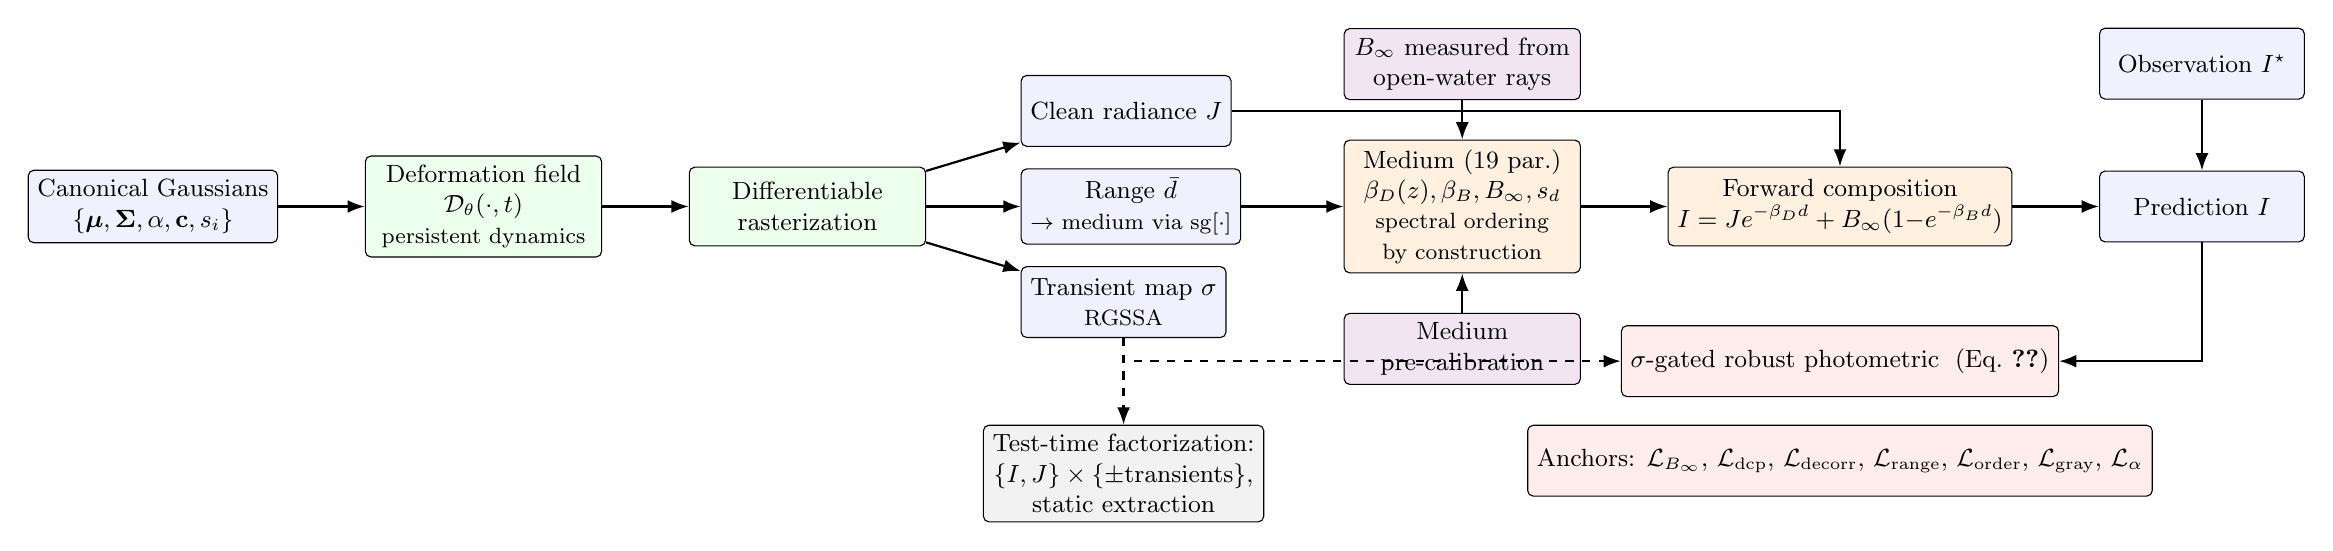
\begin{tikzpicture}[
    font=\small,
    node distance=0.9cm and 1.1cm,
    data/.style={draw, rounded corners=2pt, align=center, minimum width=2.6cm, minimum height=0.9cm, fill=blue!6},
    module/.style={draw, rounded corners=2pt, align=center, minimum width=3.0cm, minimum height=1.0cm, fill=green!7},
    medium/.style={draw, rounded corners=2pt, align=center, minimum width=3.0cm, minimum height=1.0cm, fill=orange!12},
    measure/.style={draw, rounded corners=2pt, align=center, minimum width=3.0cm, minimum height=0.9cm, fill=violet!10},
    objective/.style={draw, rounded corners=2pt, align=center, minimum width=3.4cm, minimum height=0.9cm, fill=red!7},
    output/.style={draw, rounded corners=2pt, align=center, minimum width=2.7cm, minimum height=0.9cm, fill=gray!10},
    arrow/.style={-{Latex[length=2.2mm]}, thick},
    dashedarrow/.style={-{Latex[length=2.2mm]}, thick, dashed}
]

% Scene branch
\node[data] (canon) {Canonical Gaussians\\$\{\boldsymbol{\mu},\boldsymbol{\Sigma},\alpha,\mathbf{c},s_i\}$};
\node[module, right=of canon] (deform) {Deformation field\\$\mathcal{D}_\theta(\cdot, t)$\\\footnotesize persistent dynamics};
\node[module, right=of deform] (rast) {Differentiable\\rasterization};

\node[data, above right=0.25cm and 1.2cm of rast] (J) {Clean radiance $\J$};
\node[data, right=1.2cm of rast] (range) {Range $\bar d$\\\footnotesize $\to$ medium via $\sg[\cdot]$};
\node[data, below right=0.25cm and 1.2cm of rast] (sigma) {Transient map $\sigma$\\\footnotesize RGSSA};

% Medium branch
\node[medium, right=1.3cm of range] (med) {Medium (19 par.)\\$\beta_D(z),\beta_B,\Binf,s_d$\\\footnotesize spectral ordering\\\footnotesize by construction};
\node[measure, above=0.5cm of med] (binfm) {$\Binf$ measured from\\open-water rays};
\node[measure, below=0.5cm of med] (precal) {Medium\\pre-calibration};

\node[medium, right=of med] (comp) {Forward composition\\$\I = \J e^{-\beta_D d} + \Binf(1{-}e^{-\beta_B d})$};

\node[data, right=of comp] (Ipred) {Prediction $\I$};
\node[data, above=of Ipred] (gt) {Observation $\I^\star$};

% Objectives
\node[objective, below=1.0cm of comp] (photo) {$\sigma$-gated robust photometric\; (Eq.~\ref{eq:robust})};
\node[objective, below=0.35cm of photo] (anchors) {Anchors: $\Lcal_{\Binf}$, $\Lcal_{\text{dcp}}$, $\Lcal_{\text{decorr}}$, $\Lcal_{\text{range}}$, $\Lcal_{\text{order}}$, $\Lcal_{\text{gray}}$, $\Lcal_{\alpha}$};

% Outputs
\node[output, below=1.1cm of sigma] (outs) {Test-time factorization:\\$\{\I,\J\}\times\{\pm\text{transients}\}$,\\static extraction};

\draw[arrow] (canon) -- (deform);
\draw[arrow] (deform) -- (rast);
\draw[arrow] (rast) -- (J);
\draw[arrow] (rast) -- (range);
\draw[arrow] (rast) -- (sigma);
\draw[arrow] (J) -| (comp.north);
\draw[arrow] (range) -- (med);
\draw[arrow] (med) -- (comp);
\draw[arrow] (binfm) -- (med);
\draw[arrow] (precal) -- (med);
\draw[arrow] (comp) -- (Ipred);
\draw[arrow] (gt) -- (Ipred);
\draw[arrow] (Ipred) |- (photo.east);
\draw[dashedarrow] (sigma.south) |- (photo.west);
\draw[dashedarrow] (sigma) -- (outs);

\end{tikzpicture}
}
\caption{\textbf{PhysDecouple-4DGS.} The deformable scene renders clean radiance $\J$, range $\bar d$, and the transient map $\sigma$ in one pass. The 19-parameter medium --- veiling light measured from open-water rays, attenuation and backscatter spectrally ordered by construction, pre-calibrated before joint optimization --- composites the underwater prediction $\I$ supervised against $\I^\star$ through the $\sigma$-gated robust photometric loss and ungated anchor objectives. Test-time gates over $\sigma$ and deformation magnitude factorize reconstruction/restoration with/without transients and a fully static extraction.}
\label{fig:architecture}
\end{figure}

\section{Experiments}

\paragraph{Setup.} We evaluate on three dynamic coastal video scenes (300 frames each, held-out test views by the standard 1-in-8 protocol) and the four SeaThru-NeRF photo collections, against six recent underwater novel-view baselines: SeaThru-NeRF \cite{levy2023seathru}, WaterSplatting \cite{li2025watersplatting}, SeaSplat \cite{yang2025seasplat}, RUSplatting \cite{jiang2025rusplatting}, UW-GS \cite{wang2025uwgs}, and Plenodium \cite{wu2025plenodium}, all retrained on the same data. A single PhysDecouple-4DGS configuration is used for every scene --- no per-scene tuning. On the dynamic scenes our reconstruction reaches PSNR 33.2 / 30.0 / 27.5 dB (SSIM 0.89 / 0.84 / 0.77).

\paragraph{Metrics.} Reconstruction is evaluated full-reference on held-out views (PSNR, SSIM \cite{wang2004image}, LPIPS \cite{zhang2018unreasonable}). Restoration has no clean reference, so we report the standard no-reference underwater quality measures UIQM \cite{panetta2015no} and UCIQE \cite{yang2013unsupervised}. Table~\ref{tab:quant} reports all methods on all scenes; the first and second best entries per metric are highlighted in red and blue, respectively.

\begin{table}[t]
\centering
\small
\begin{tabular}{llccccc}
\toprule
Scene & Method & PSNR$\uparrow$ & SSIM$\uparrow$ & LPIPS$\downarrow$ & UIQM$\uparrow$ & UCIQE$\uparrow$ \\
\midrule
set4 & SeaThru-NeRF & \second{31.663} & 0.835 & 0.239 & 1.091 & 0.181 \\
 & WaterSplatting & 30.113 & 0.845 & 0.238 & 1.864 & \first{0.320} \\
 & SeaSplat & 17.451 & 0.871 & \first{0.130} & 1.210 & \second{0.302} \\
 & RUSplatting & 31.616 & \second{0.876} & 0.209 & 1.998 & 0.242 \\
 & UW-GS & 28.341 & 0.811 & 0.317 & 1.521 & 0.219 \\
 & Plenodium & 30.209 & 0.849 & 0.248 & \second{2.045} & 0.238 \\
 & \textbf{Ours} (v14) & \first{33.231} & \first{0.891} & \second{0.159} & \first{2.475} & 0.259 \\
\midrule
set5 & SeaThru-NeRF & \second{29.072} & 0.735 & 0.238 & 3.096 & 0.160 \\
 & WaterSplatting & 27.936 & 0.765 & 0.211 & 3.767 & \first{0.311} \\
 & SeaSplat & 13.269 & 0.761 & \second{0.146} & 2.244 & 0.219 \\
 & RUSplatting & 29.034 & \second{0.810} & 0.162 & \first{4.319} & 0.242 \\
 & UW-GS & 25.187 & 0.648 & 0.333 & 3.204 & 0.195 \\
 & Plenodium & 28.004 & 0.764 & 0.224 & \second{4.224} & \second{0.306} \\
 & \textbf{Ours} (v15) & \first{31.402} & \first{0.864} & \first{0.104} & 4.028 & 0.179 \\
\midrule
set8 & SeaThru-NeRF & 26.955 & 0.670 & 0.329 & 3.291 & 0.195 \\
 & WaterSplatting & 26.410 & 0.690 & 0.247 & \second{4.326} & 0.255 \\
 & SeaSplat & 13.477 & \first{0.840} & \first{0.091} & 3.854 & 0.253 \\
 & RUSplatting & \second{28.015} & 0.780 & 0.191 & 4.274 & 0.237 \\
 & UW-GS & 24.242 & 0.583 & 0.432 & 2.661 & 0.253 \\
 & Plenodium & 26.331 & 0.691 & 0.260 & 4.078 & \first{0.262} \\
 & \textbf{Ours} (v15) & \first{28.535} & \second{0.801} & \second{0.171} & \first{4.403} & \second{0.258} \\
\bottomrule
\end{tabular}

\caption{\textbf{Quantitative comparison.} Full-reference reconstruction metrics (PSNR/SSIM/LPIPS, against held-out underwater frames) and no-reference restoration metrics (UIQM/UCIQE, on the restored outputs). The \textcolor{firstbest}{\textbf{first best}} and \textcolor{secondbest}{\textbf{second best}} results are highlighted in red and blue, respectively.}
\label{tab:quant}
\end{table}

\paragraph{Restoration (UIR).} Figures~\ref{fig:uir4}--\ref{fig:uir8} compare restored outputs. Zoomed regions (yellow: scene detail; red: far field) show the two regimes where prior methods degrade: detail loss in the restored output, and depth-graded color casts in the far field. Our restoration preserves detail at the level of the reconstruction and maintains a range-independent color balance.

\paragraph{Novel-view reconstruction (NVS).} Figures~\ref{fig:nvs4}--\ref{fig:nvs8} compare reconstructions of held-out views against the underwater ground truth.

\paragraph{Model factorization.} Figure~\ref{fig:decomp} shows the full per-view factorization produced by one trained model on our main dynamic scenes (S5, S4, S8) --- reconstruction, restoration, transient-suppressed restoration, backscatter, transient probability, and range --- the output set that constitutes the transient-removal and restoration deliverables. We show similar per-view factorizations for the SeaThru-NeRF collections and NUSR datasets in Figure~\ref{fig:decomp_seathru} and Figure~\ref{fig:decomp_nusr}. No baseline provides this factorization for dynamic scenes.

\textit{[Pending final rounds: quantitative tables for all methods/scenes, the measured-$\hat\Binf$ table, and ablations (decorrelation, $\Binf$ measurement, robust gating, ordering).]}

\begin{figure}[p]
\centering
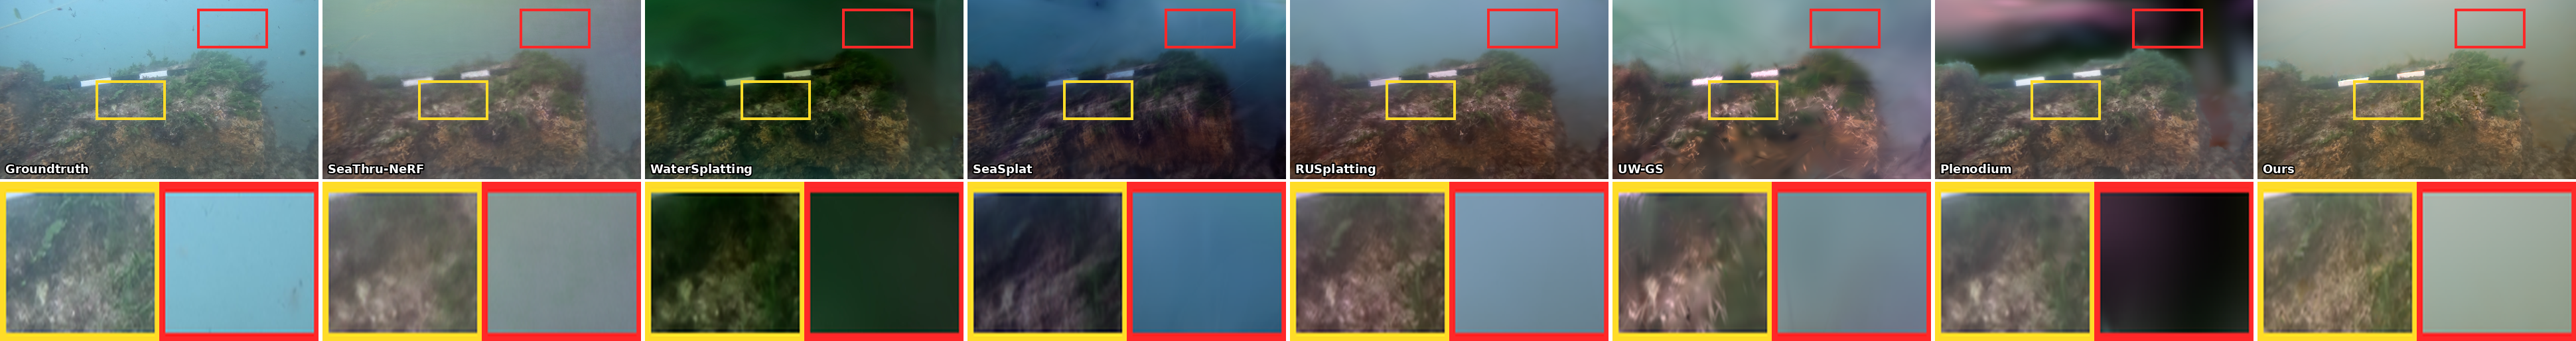
\includegraphics[width=\textwidth]{assets/results/set4_uir.png}
\caption{\textbf{Underwater image restoration, Scene S4.} Columns: ground truth and seven methods; below each: zoomed yellow (detail) and red (far-field) crops. Competing restorations lose contrast or shift hue with distance; ours stays color-stable across range.}
\label{fig:uir4}
\end{figure}

\begin{figure}[p]
\centering
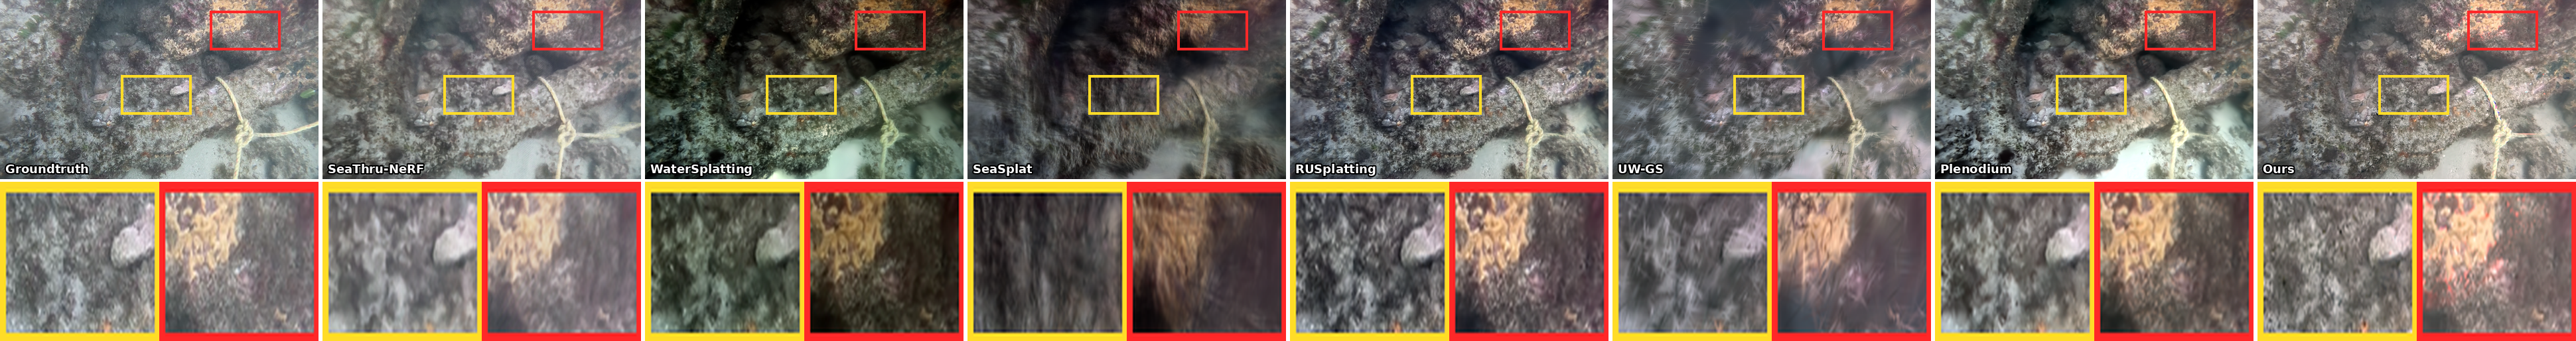
\includegraphics[width=\textwidth]{assets/results/set5_uir.png}
\caption{\textbf{Underwater image restoration, Scene S5} (dynamic rope, transient fish). Our output additionally has transients suppressed.}
\label{fig:uir5}
\end{figure}

\begin{figure}[p]
\centering
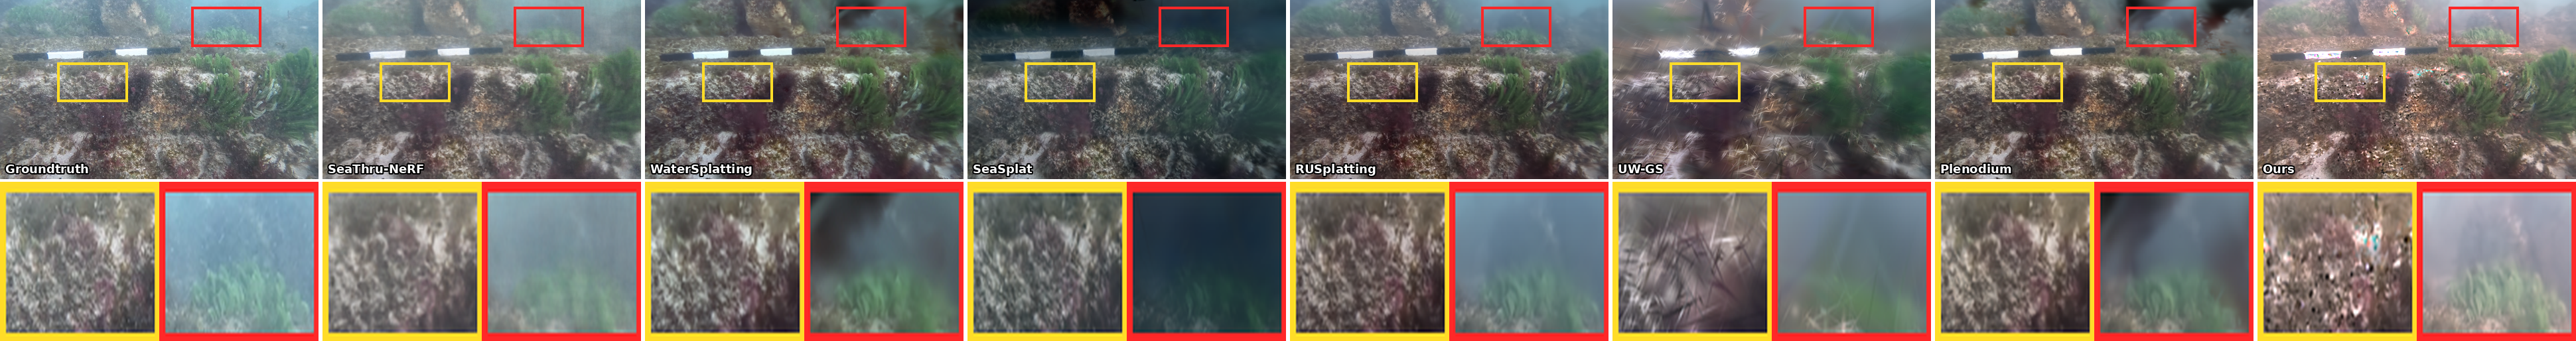
\includegraphics[width=\textwidth]{assets/results/set8_uir.png}
\caption{\textbf{Underwater image restoration, Scene S8} (heavy veiling). The far-field crop (red) isolates veil handling.}
\label{fig:uir8}
\end{figure}

\begin{figure}[p]
\centering
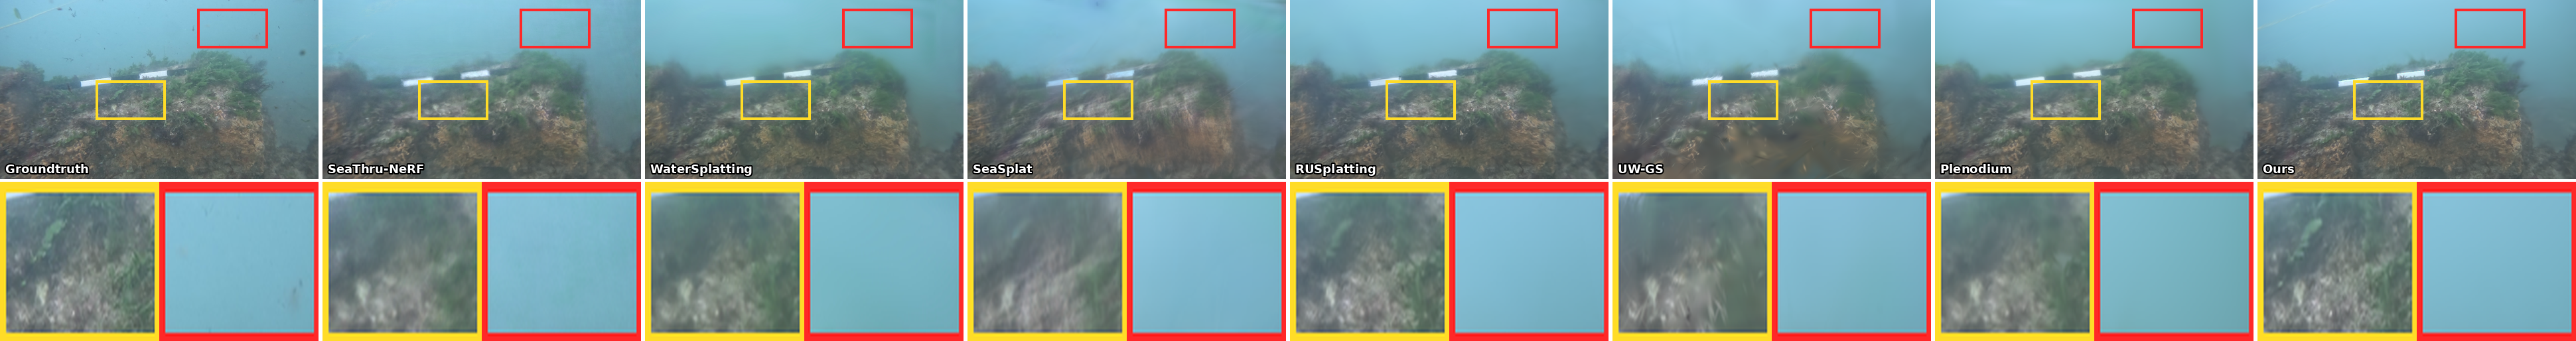
\includegraphics[width=\textwidth]{assets/results/set4_nvs.png}
\caption{\textbf{Novel-view reconstruction, Scene S4.}}
\label{fig:nvs4}
\end{figure}

\begin{figure}[p]
\centering
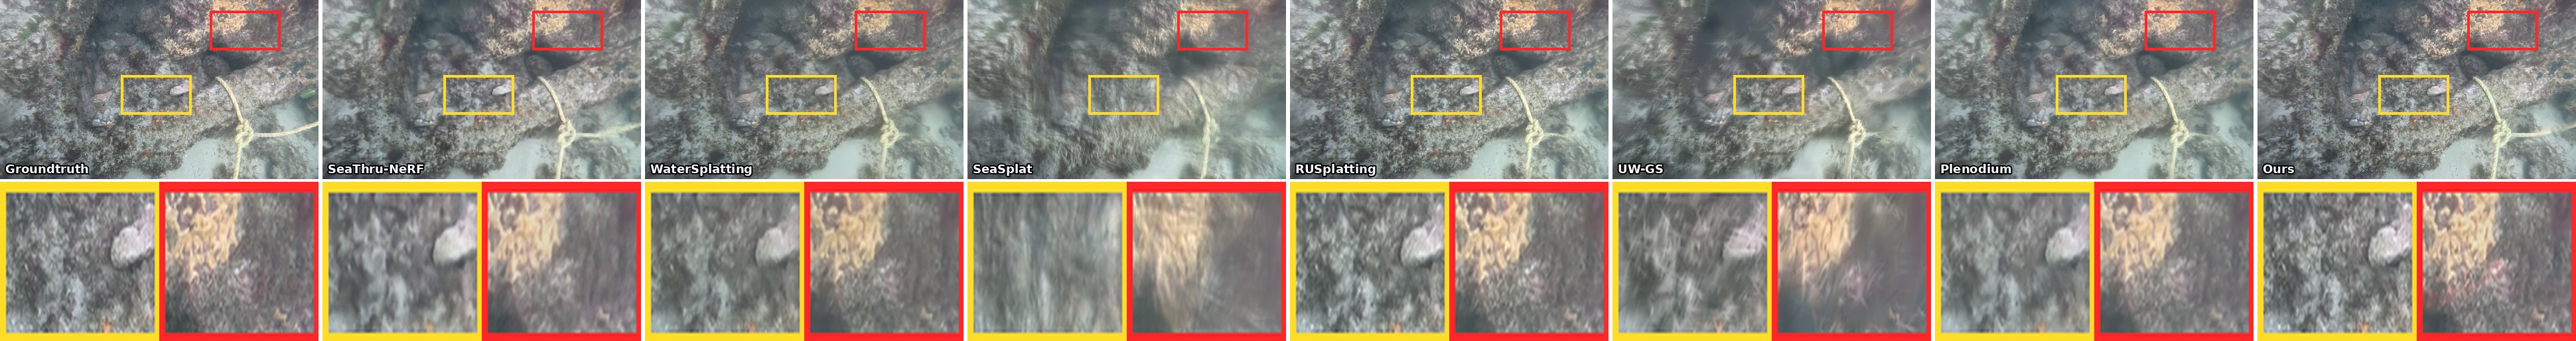
\includegraphics[width=\textwidth]{assets/results/set5_nvs.png}
\caption{\textbf{Novel-view reconstruction, Scene S5.}}
\label{fig:nvs5}
\end{figure}

\begin{figure}[p]
\centering
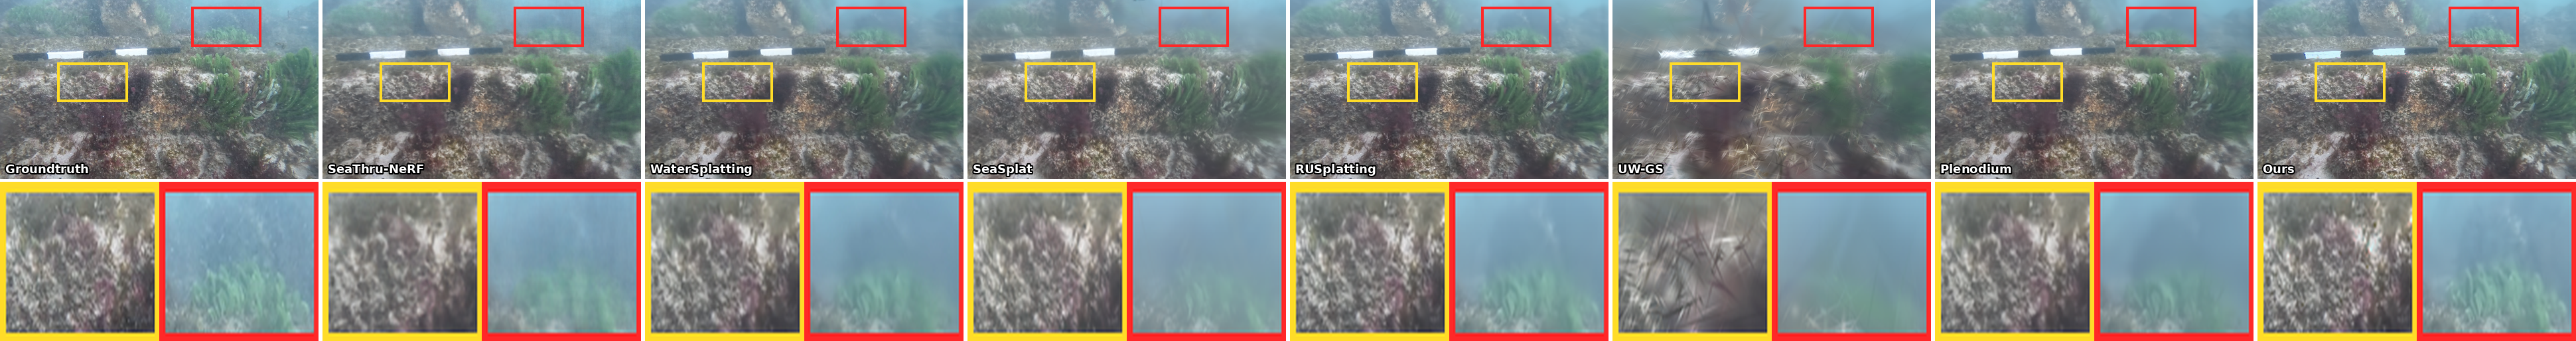
\includegraphics[width=\textwidth]{assets/results/set8_nvs.png}
\caption{\textbf{Novel-view reconstruction, Scene S8.}}
\label{fig:nvs8}
\end{figure}

\begin{figure}[p]
\centering
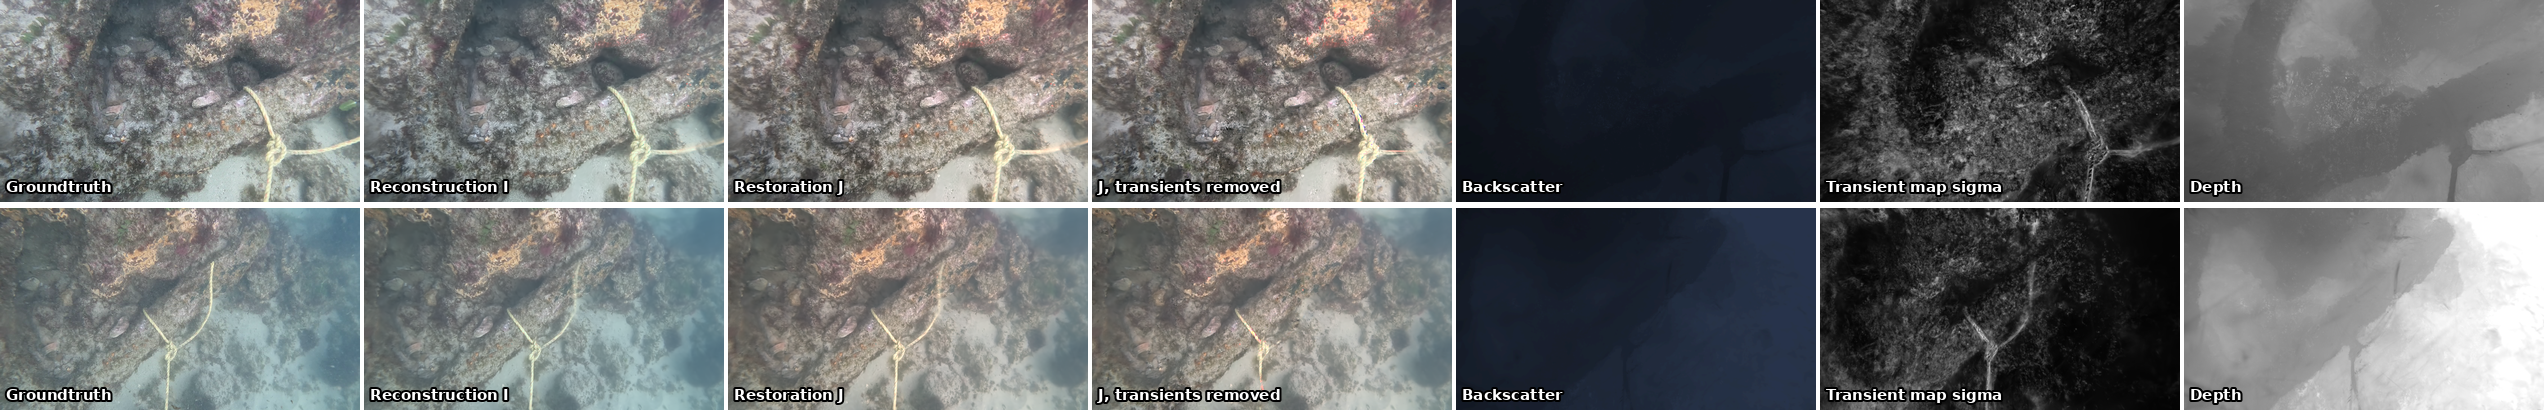
\includegraphics[width=\textwidth]{assets/results/set5_decomposition.png}\\[4pt]
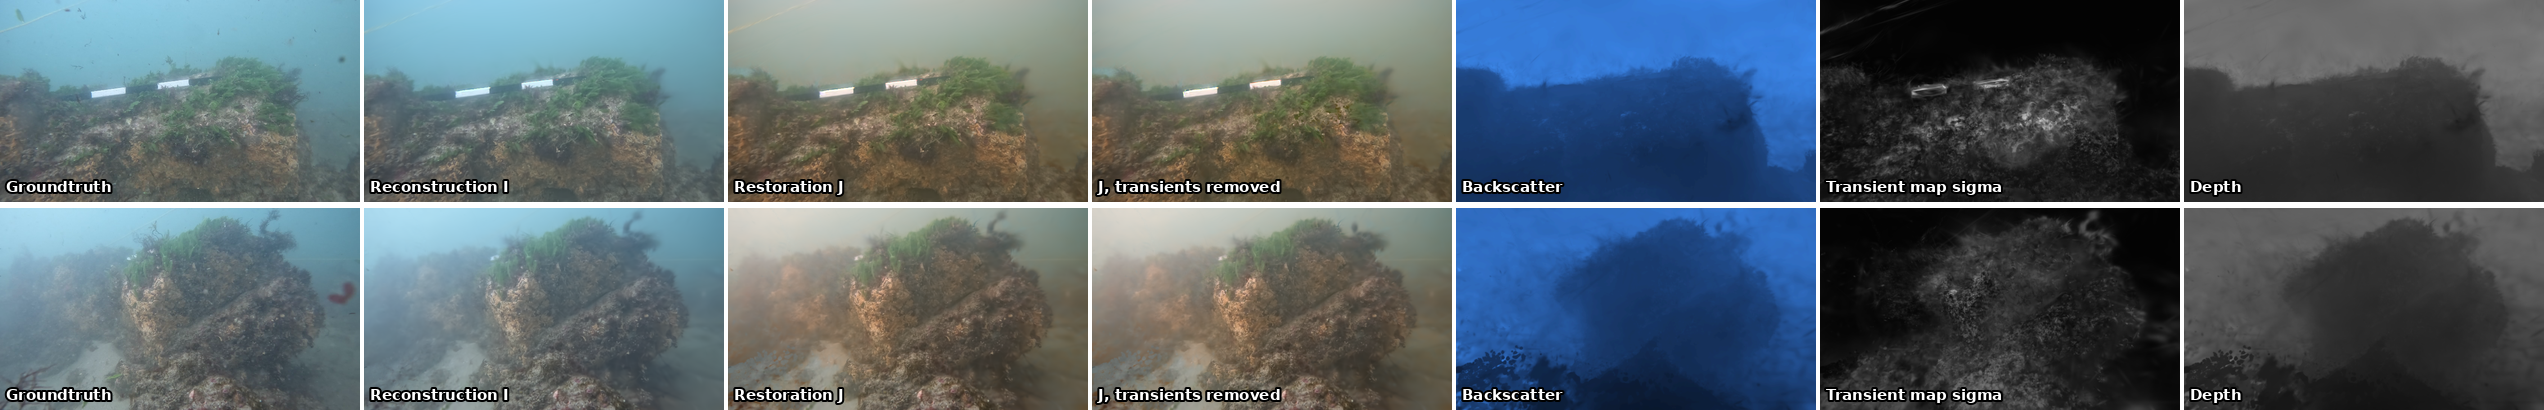
\includegraphics[width=\textwidth]{assets/results/set4_decomposition.png}\\[4pt]
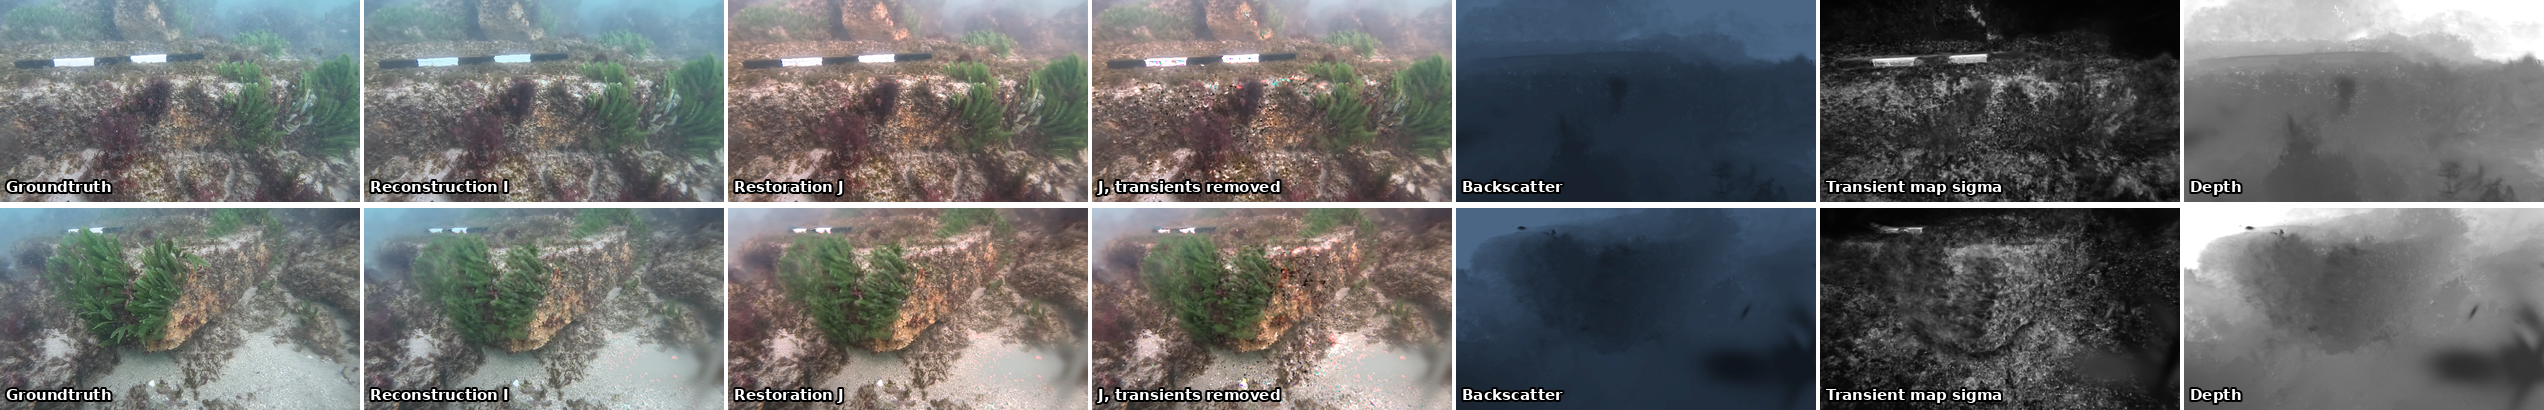
\includegraphics[width=\textwidth]{assets/results/set8_decomposition.png}
\caption{\textbf{Per-view factorization} (two views per scene; S5, S4, S8): ground truth, reconstruction $\I$, restoration $\J$, transient-suppressed restoration, backscatter (display-normalized $\times 3$), transient probability $\sigma$, and range. The $\sigma$ map concentrates on transients and unstable thin structure; backscatter follows range as the physics requires.}
\label{fig:decomp}
\end{figure}

\begin{figure}[p]
\centering
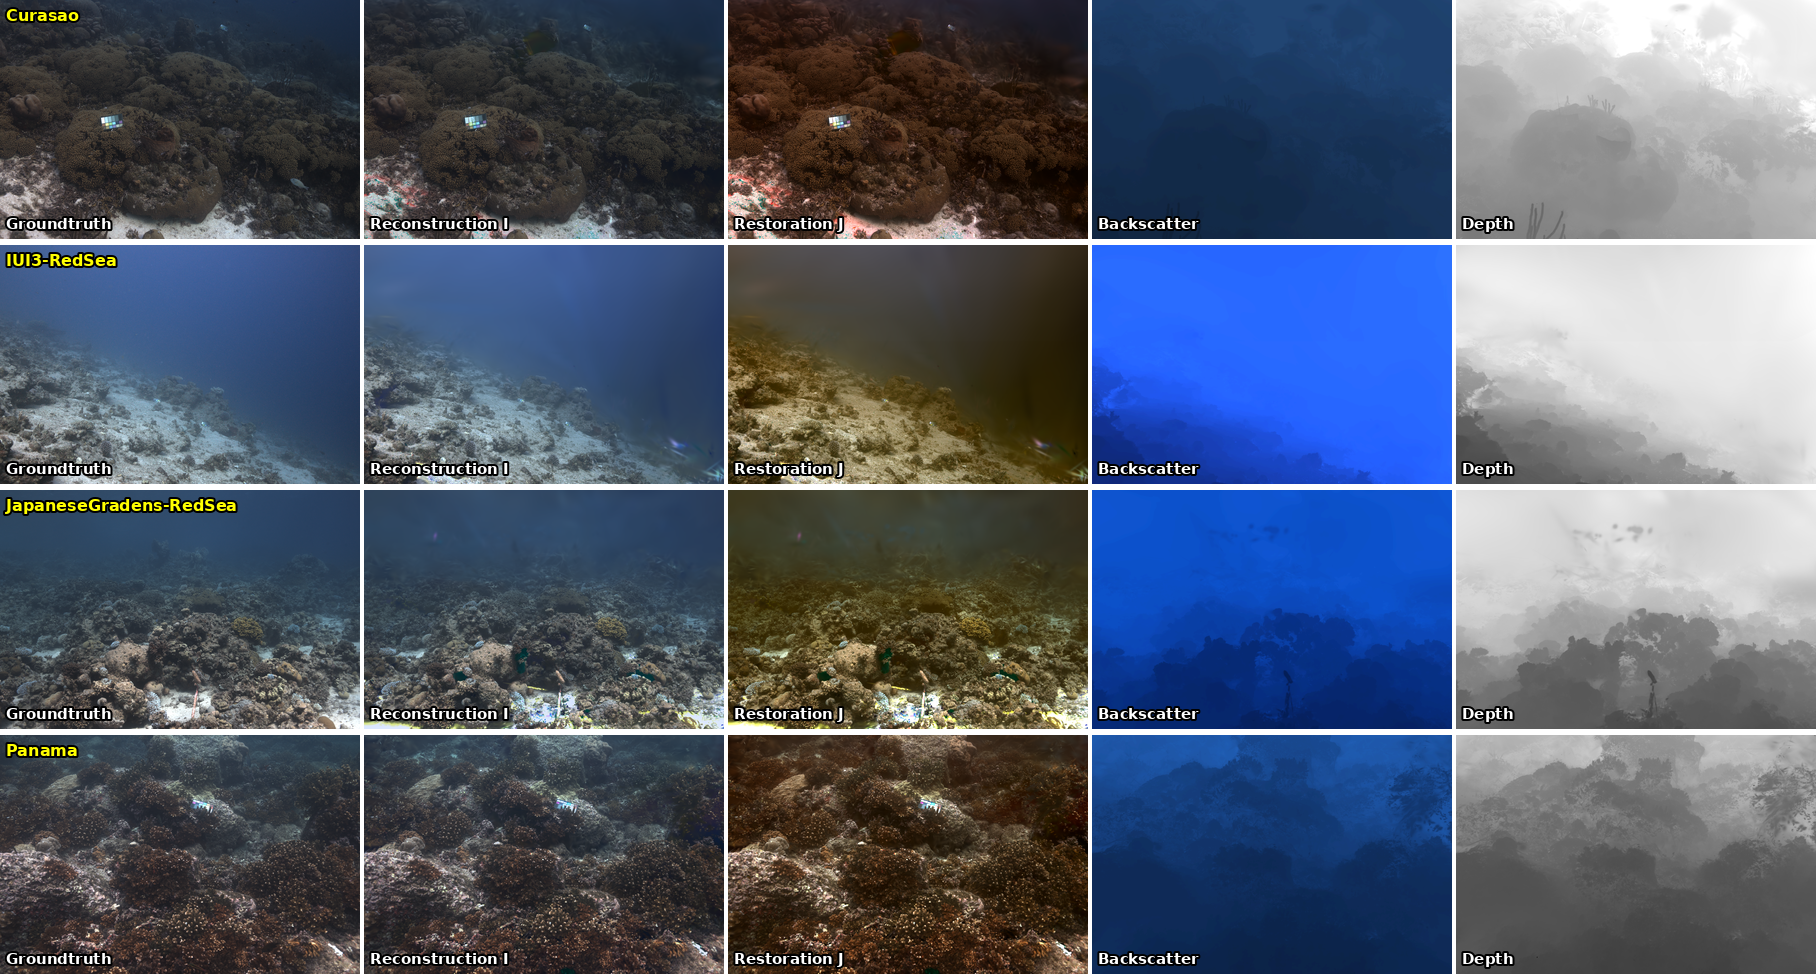
\includegraphics[width=\textwidth]{assets/results/seathrunerf_decomposition.png}
\caption{\textbf{Model factorization on the SeaThru-NeRF dataset.} Factorization results for Curasao, IUI3-RedSea, JapaneseGradens-RedSea, and Panama scenes: ground truth, reconstruction $\I$, restoration $\J$, backscatter (display-normalized $\times 3$), and range. The restoration preserves fine details while range-dependent veils are cleanly decoupled.}
\label{fig:decomp_seathru}
\end{figure}

\begin{figure}[p]
\centering
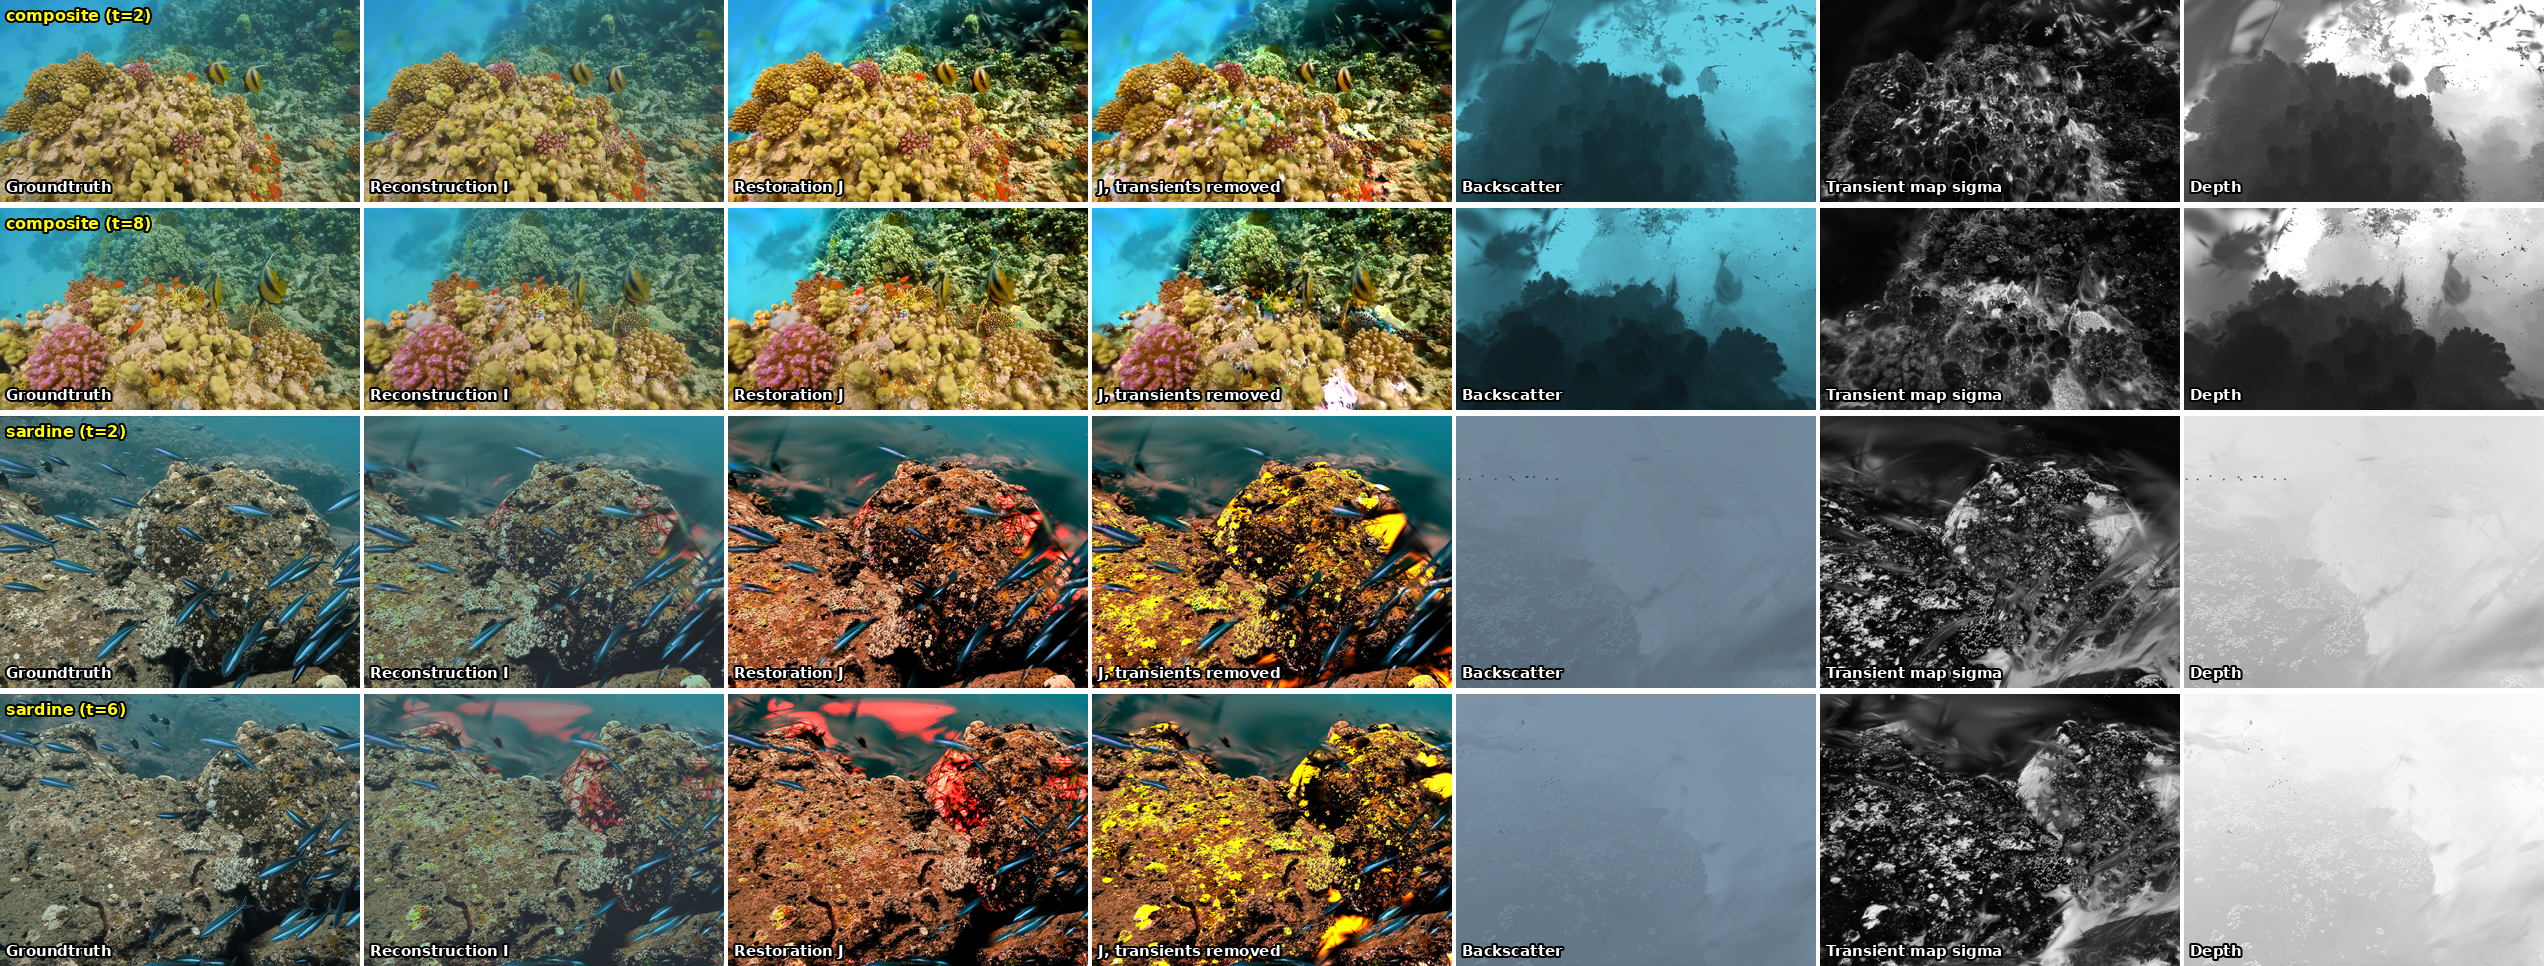
\includegraphics[width=\textwidth]{assets/results/nusr_decomposition.png}
\caption{\textbf{Model factorization on the NUSR dataset.} Factorization results for composite and sardine scenes (two views shown per scene): ground truth, reconstruction $\I$, restoration $\J$, transient-suppressed restoration, backscatter (display-normalized $\times 3$), transient map $\sigma$, and range.}
\label{fig:decomp_nusr}
\end{figure}

\section{Limitations}
\label{sec:limitations}

\paragraph{Homogeneous, stationary medium.}
Replacing spatio-temporal coefficient grids with the 19-parameter medium of Sec.~\ref{sec:medium-param} is an explicit modeling decision, and it encodes two physical assumptions: the water is \emph{spatially homogeneous} over the captured volume (attenuation varies with range but not laterally; backscatter and veiling light are scene constants) and \emph{stationary} over the capture interval. These assumptions are what make the inverse problem identifiable --- a medium with thousands of free coefficients is observationally indistinguishable from scene appearance, and in our experiments grid-based media absorbed scene content and noise --- but they bound the method's applicability. Scenes with localized turbidity (sediment plumes, thermoclines), artificial illumination (strobes, dive lights, pronounced sun shafts and caustics), or conditions that drift over long captures violate them; extending the medium with low-dimensional, physically structured spatial or temporal components (e.g., a depth-stratified veil or a slowly varying illumination scalar) without re-opening the identifiability gap is left to future work.

\paragraph{Veiling-light observability.}
The $\Binf$ measurement requires open water in the field of view. Where none is visible, the method falls back to the dark-pixel estimator, which is biased in bright, shallow scenes; the calibration anchor mitigates but does not eliminate this.

\paragraph{Water-class bounds.}
Attenuation and backscatter coefficients are bounded within a user-selected Jerlov class. The bounds are physically motivated and the parameters are learned within them, but a strongly atypical medium (e.g., algal bloom) may fall outside the chosen locus.

\paragraph{Depth and motion priors.}
Range supervision relies on monocular depth, which is non-metric and can be unreliable on texture-poor water regions; the formation model consumes rendered range, so systematic range bias maps to medium bias. The transient taxonomy assigns slow, persistent movers to the deformation field by construction; objects at the boundary (e.g., an animal that lingers, then leaves) may be split between the dynamic and transient channels.

\section{Conclusion}

PhysDecouple-4DGS factorizes monocular underwater video into a deformable clean scene, a compact physically constrained medium, and a transient layer, by combining direct underwater rendering with measurement-first medium estimation and a small set of identifiability constraints, each tied to a physical property of the problem: spectral orderings hold by construction; the veiling light is observed, not assumed; transmission is bounded away from unobservability; and the range-independence of restored chromaticity --- a necessary condition for any correct restoration --- supervises the reconstruction directly. A single configuration trains stably across coastal video and deep oceanic photo collections, and one trained model serves reconstruction, restoration, transient removal, and static-scene extraction. We believe the identifiability analysis and the measurement-first methodology extend beyond water to other participating media composited over splatting-based scene representations.

\appendix

\section{Physical and Mathematical Intuition}
\label{sec:appendix_intuition}

This appendix details the underlying physical reasoning, mathematical formulation, and optimization design choices for \texttt{PhysDecouple-4DGS}, as motivated by constraints identified in training telemetry and the physical characteristics of participating media.

\subsection{19-Parameter Medium Parameterization}
The optical model is deliberately restricted to 19 scalar parameters to prevent the high-capacity scene representation from trade-offs with medium parameters. The 19 parameters are:
\begin{enumerate}
    \item \textbf{Direct Attenuation $\beta_D^c(z)$ (12 parameters)}: Modeled as a two-term exponential per color channel $c \in \{R,G,B\}$:
    \begin{equation}
        \beta_D^c(z) = a_c e^{b_c z} + c_c e^{d_c z}
    \end{equation}
    where monotonicity of decay is enforced by reparameterizing $a_c, c_c > 0$ via a softplus function and $b_c, d_c < 0$ via a negated softplus function. This formulation ensures that light decay is physically plausible and smooth without spatial grid representations.
    
    \item \textbf{Backscatter Coefficient $\beta_B$ (3 parameters)}: Modeled as a scene-constant RGB triple, since oceanographic data indicates it varies weakly with object distance $z$.
    
    \item \textbf{Veiling Light $B_{\infty}$ (3 parameters)}: Modeled as a scene-constant RGB triple, capturing the asymptotic background radiance.
    
    \item \textbf{Learned Depth Scale $s_d$ (1 parameter)}: Monocular depth map estimations are non-metric. We map normalized depth $\bar{d} \in [0, 1]$ to physical path length $d = s_d \bar{d}$, where $s_d \in [0.5, 4.0]$. The upper limit prevents transmission from falling below $e^{-2.4} \approx 0.09$, ensuring the clean radiance $J$ receives non-trivial photometric gradients even at far-field distances.
\end{enumerate}

\subsection{Hard Spectral Orderings by Construction}
To prevent unphysical color estimation (e.g., green water behaving as deep-blue open ocean), we enforce physical spectral ordering by sequential bounded reparameterization:
\begin{itemize}
    \item \textbf{Direct Attenuation}: Red light attenuates fastest ($\beta_D^R > \beta_D^G > \beta_D^B$), enforced by:
    \begin{equation}
        \beta_D^G(z) = \min\left(\beta_D^G(z),\, \beta_D^R(z) - \varepsilon\right), \quad \beta_D^B(z) = \min\left(\beta_D^B(z),\, \beta_D^G(z) - \varepsilon\right)
    \end{equation}
    \item \textbf{Backscatter and Veiling Light}: Blue scatters most ($\beta_B^B > \beta_B^G > \beta_B^R$ and $B_{\infty}^B > B_{\infty}^G > B_{\infty}^R$), enforced similarly:
    \begin{equation}
        \beta_B^G = \max\left(\beta_B^G,\, \beta_B^R + \varepsilon\right), \quad \beta_B^B = \max\left(\beta_B^B,\, \beta_B^G + \varepsilon\right)
    \end{equation}
\end{itemize}
These bounds prevent the optimization from violating basic optical physics under severe noise or lack of visual cues.

\subsection{Range Stop-Gradient Intuition}
Allowing gradients to flow back through the medium exponent $e^{-\beta_D d}$ into the depth maps $\bar{d}$ creates a degenerate shortcut termed ``depth painting.'' Because changing depth modulates colors exponentially, the optimizer shifts geometry to minimize color discrepancy, causing the Gaussians to fragment into disjoint floaters that paint colors at arbitrary depths. Detaching gradients $\text{sg}[\bar{d}]$ ensures that geometry is supervised solely by the radiance pathways and explicit range losses, maintaining clean, continuous surfaces.

\subsection{Depth--Chromaticity Decorrelation Loss}
The physical formation model dictates that the water medium is the only factor introducing range-dependent color shifts. Therefore, a clean restoration $J$ must satisfy color constancy: its chromaticity must be statistically independent of range. We supervise this using Pearson correlation $\rho$ on log-chromaticities $u, v$:
\begin{equation}
    \mathcal{L}_{\text{decorr}} = \frac{1}{2}\left[ \left(|\rho(\bar{d}, u)| - \tau_{\rho}\right)_+ + \left(|\rho(\bar{d}, v)| - \tau_{\rho}\right)_+ \right], \quad \tau_{\rho} = 0.10
\end{equation}
The margin $\tau_{\rho}$ accommodates minor natural color changes across distance while preventing global shifts (such as yellow/blue far-field casts) where the photometric gradient is weak.

\subsection{Residual-Guided Spatial Sigma Assignment (RGSSA)}
Standard deformation-based transient modeling only detects moving Gaussians whose displacements can be tracked. Slowly drifting fish, floating particles, and water bubbles are often incorrectly absorbed into the deformation field or geometry. RGSSA addresses this by routing the model's own photometric rendering residuals $R(\mathbf{x}) = |I(\mathbf{x}) - I^\star(\mathbf{x})|$ directly to supervise the transient map $\sigma(\mathbf{x})$:
\begin{equation}
    \mathcal{L}_{\sigma\text{-res}} = \|\sigma(\mathbf{x}) - \phi(R(\mathbf{x}))\|_1
\end{equation}
Where the forward medium model and deformation field fail to consistently explain a pixel, it is self-supervised as transient, gating the photometric loss to protect the static representation.

\subsection{Optimization and Learning Rate Scheduling}
Naively training the high-capacity scene model and the compact medium jointly causes the scene model to absorb the initialization mismatch. We resolve this by freezing the scene at the handoff and pre-calibrating the medium alone for 400 steps. During joint training, the medium parameters are updated at a rate of $5\times 10^{-3}$ (an order of magnitude faster than standard neural fields) with a gradient clip at $1.0$. This ensures the medium dynamically tracks changes, and the scene model reconstructs details around a stable water column.

\bibliographystyle{plain}
\bibliography{references}

\end{document}
